\documentclass[10pt,twocolumn,a4paper]{article}

% -------------------------------------------------
% Language and encoding
% -------------------------------------------------
\usepackage[T1]{fontenc}
\usepackage{lmodern}
\usepackage[english]{babel}

% -------------------------------------------------
% Document format
% -------------------------------------------------
\usepackage[
    top=1.8cm,
    bottom=1.8cm,
    left=1.8cm,
    right=1.8cm,
    columnsep=0.7cm
]{geometry}

\usepackage{microtype}
\usepackage{parskip}
\usepackage{ragged2e}

% -------------------------------------------------
% Mathematics
% -------------------------------------------------
\usepackage{amsmath}
\usepackage{amssymb}
\usepackage{bm}

% -------------------------------------------------
% Figures and tables
% -------------------------------------------------
\usepackage{graphicx}
\usepackage{booktabs}
\usepackage{array}
\usepackage{siunitx}
\usepackage{float}
\usepackage{placeins}

\setlength{\intextsep}{8pt}
\setlength{\textfloatsep}{8pt}
\setlength{\floatsep}{8pt}

% -------------------------------------------------
% Links and references
% -------------------------------------------------
\usepackage[hidelinks]{hyperref}

% Folder containing the regression figure extracted from the notes
\graphicspath{{images/}}

% -------------------------------------------------
% Document information
% -------------------------------------------------
\title{
    \textbf{Learning from an Expert Controller:\\
    Supervised Dataset Generation\\
    and Linear Velocity Regression}
}

\author{
    Julio Quejido Barrera\\
    Humanoide Robotik\\
    Julio's Laboratories
}

\date{\today}

% =================================================
\begin{document}
% =================================================

\maketitle
\raggedbottom

\begin{abstract}
This project describes the transition from mobile-robot navigation programmed
through geometric rules and reactive controllers to a first supervised-learning
workflow. In the dataset-generation stage, the existing controller is used as
an expert that assigns an action to many independently sampled robot
situations. Each valid sample stores the robot state, goal information, sensor
readings, and the expert commands. The resulting dataset is then used to fit a
simple linear-regression model that attempts to learn the relationship between
distance to the goal and linear velocity. The purpose is not yet to obtain a
complete learned controller, but to understand the supervised-learning
pipeline: how robot behavior is represented as input-output data, how a linear
model is fitted from examples, how its parameters are computed, and how the
prediction error is evaluated. The experiment also demonstrates why a single
linear feature cannot reproduce an expert policy that contains speed
saturation and rule-based obstacle-avoidance decisions.
\end{abstract}

\section{Introduction}

In the previous navigation experiments, the robot action was produced directly
from geometric quantities, sensor readings, and programmed control rules. The
information flow was

\[
    \text{current state}
    \longrightarrow
    \text{programmed rules}
    \longrightarrow
    \text{robot action}.
\]

The present project introduces a different objective. Instead of applying the
controller only to move the robot, the controller is treated as an
\emph{expert} that generates examples. Those examples are stored and later
used to fit a model. The workflow becomes

\[
    \text{current state}
    \longrightarrow
    \text{stored expert action}
    \longrightarrow
    \text{learned model}.
\]

The central input-output relationship is

\[
    \text{robot state + sensors + goal}
    \longrightarrow
    \text{expert action}.
\]

The generated dataset contains many examples of this mapping. The first
learning experiment then uses only a small part of the available information:
the distance to the goal is used as the input variable, and the expert linear
velocity is used as the output to be predicted. This deliberately simple
regression problem makes it possible to study what a straight line can learn
and which parts of the expert policy it cannot represent.

\section{Supervised Dataset Generation}

\subsection{Objective of the Experiment}

The objective of the dataset-generation stage is to produce a supervised
dataset for mobile robotics. Each row represents one valid robot situation and
the action that the expert controller would choose in that situation. Unlike a
trajectory simulation, the robot is not propagated from one state to the next.
Instead, many independent states are sampled and evaluated.

Each example has the generic form

\[
    \text{features}
    \longrightarrow
    \text{labels}.
\]

For this project, the relationship can be summarized as

\[
\begin{bmatrix}
    \text{robot position}\\
    \text{orientation}\\
    \text{goal}\\
    \text{distance to goal}\\
    \text{angular error}\\
    \text{sensor readings}
\end{bmatrix}
\longrightarrow
\begin{bmatrix}
    v\\
    \omega
\end{bmatrix}.
\]

Thus, the dataset connects the state and perception of the robot with the
control action selected by the expert.

\subsection{Elements Reused from Reactive Navigation}

The geometric and control basis was developed in the previous navigation
project: Euclidean goal distance, normalized angular error, proportional
angular control, saturated linear speed, range sensors, circular obstacles,
ray projection, and ray-circle intersection. In the present experiment these
elements are reused, but their role changes from producing motion to producing
stored supervised examples.

\begin{table*}[!t]
\centering
\small
\caption{Previously developed navigation elements and their role in dataset generation.}
\label{tab:reused_elements}
\begin{tabular}{>{\raggedright\arraybackslash}p{0.18\textwidth}
                >{\raggedright\arraybackslash}p{0.35\textwidth}
                >{\raggedright\arraybackslash}p{0.39\textwidth}}
\toprule
\textbf{Reused element} & \textbf{Known use} & \textbf{Use in the dataset} \\
\midrule
Distance to the goal
& $d=\lVert\mathbf{p}_G-\mathbf{p}\rVert$.
& Stored as a feature. Samples inside the goal tolerance are discarded and replaced. \\

Normalized angular error
& Shortest signed rotation toward the goal, $e_\theta=\operatorname{norm}(\theta_G-\theta)$.
& Stored as a feature in radians. \\

Proportional angular control
& Produces $\omega=K_\theta e_\theta$.
& Generates the label $\omega$ instead of updating the robot pose; the command is limited by $\omega_{\max}$. \\

Speed with saturation
& In free space, $v=\min(K_v d,v_{\max})$.
& The resulting speed is stored as the label $v$. The saturation becomes important in the regression stage. \\

Near-goal adjustment
& Previously changed controller or sensor parameters close to the goal.
& Removed in the final dataset so that the sampling conditions remain constant; the sensor range stays fixed at $R_s=3.0$. \\

Discrete motion
& Previously updated $\mathbf{p}_{k+1}=\mathbf{p}_k+v_k\mathbf{h}_k\Delta t$ and $\theta_{k+1}=\theta_k+\omega_k\Delta t$.
& Not applied. Every row is an independent mapping from state to stored action. \\

Range sensors
& Left, right, and front finite-range sensors.
& Only one scalar distance is stored for each sensor; endpoints and trajectories are not stored. \\

Circular obstacles
& Each obstacle is defined by center $\mathbf{c}_j$ and radius $r_j$.
& Random robot positions inside an obstacle are rejected as invalid states. \\

Projection onto the ray
& $\lambda_{s,j}=(\mathbf{c}_j-\mathbf{p})\cdot\mathbf{u}_s$ filters possible intersections.
& Used without noise or filtering to obtain the ideal sensor reading. \\

Ray-circle intersection
& The first valid impact distance $t_{\mathrm{near}}$ is selected.
& The hit point is not stored. Each sensor stores the minimum valid $t_{\mathrm{near}}$; if there is no hit, it stores $R_s$. \\
\bottomrule
\end{tabular}
\end{table*}

\subsection{Main Changes with Respect to the Previous Simulation}

The objective of the program changes from sequential motion to data
collection:

\[
\begin{aligned}
    \text{before: }&\quad
    \text{sensing}\rightarrow\text{decision}\rightarrow\text{motion},\\
    \text{now: }&\quad
    \text{random state}\rightarrow\text{expert decision}\\
    &\quad\longrightarrow\text{CSV row}.
\end{aligned}
\]

Independent samples are generated until $2000$ valid rows are obtained. The
goal remains fixed at

\[
    \mathbf{p}_G=
    \begin{bmatrix}
        8.0\\
        6.0
    \end{bmatrix}.
\]

Gaussian sensor noise and exponential filtering are removed. No robot
trajectory is stored; instead, the state, sensor readings, and expert action
are written to the dataset. The sensor distances become numerical input
features, while $v$ and $\omega$ become supervised labels.

\subsection{Structure of a Dataset Row}

Each row contains twelve columns. The first ten describe the robot state,
goal, and perception, while the final two store the expert action.

\begin{table}[H]
\centering
\small
\setlength{\tabcolsep}{3pt}
\caption{Variables stored in each dataset row.}
\label{tab:dataset_columns}
\begin{tabular}{>{\raggedright\arraybackslash}p{0.31\columnwidth}
                >{\raggedright\arraybackslash}p{0.55\columnwidth}}
\toprule
\textbf{Variable} & \textbf{Interpretation} \\
\midrule
\texttt{robot\_x}, \texttt{robot\_y}
& Randomly generated robot position. \\
\texttt{robot\_theta}
& Robot orientation, stored in radians. \\
\texttt{goal\_x}, \texttt{goal\_y}
& Fixed goal position $[8.0,6.0]^T$. \\
\texttt{distance\_to\_goal}
& Euclidean distance from robot to goal. \\
\texttt{angle\_error}
& Normalized angular error, stored in radians. \\
\texttt{front\_sensor}
& Front-sensor distance; equals $R_s$ if no obstacle is detected. \\
\texttt{left\_sensor}
& Left-sensor distance; equals $R_s$ if no obstacle is detected. \\
\texttt{right\_sensor}
& Right-sensor distance; equals $R_s$ if no obstacle is detected. \\
\texttt{v}
& Expert linear velocity. \\
\texttt{omega}
& Expert angular velocity, stored in radians. \\
\bottomrule
\end{tabular}
\end{table}

The compact interpretation of one row is therefore

\[
    \text{robot state and perception}
    \longrightarrow
    \text{expert action}.
\]

\subsection{Expert Policy and Behavior Cloning}

The expert combines reactive obstacle avoidance with progress toward the
goal. If any range sensor detects an obstacle, the corresponding reactive
rule is applied. Otherwise, the goal-seeking controller is used. This can be
written as

\begin{equation}
\mathbf{u}=
\begin{cases}
    \mathbf{u}_{\mathrm{avoid}},
    & D_L\lor D_R\lor D_F,\\
    \mathbf{u}_{\mathrm{goal}},
    & \neg(D_L\lor D_R\lor D_F),
\end{cases}
\label{eq:expert_policy}
\end{equation}

where $D_L$, $D_R$, and $D_F$ indicate obstacle detections from the left,
right, and front sensors.

The reactive branch assigns discrete speed and turning commands. In free
space, the expert linear velocity follows the saturated proportional law

\begin{equation}
    v_{\mathrm{goal}}
    =
    \min(K_v d,v_{\max}).
    \label{eq:saturated_speed}
\end{equation}

The angular velocity is produced by proportional control and clipped to the
permitted interval:

\begin{equation}
\omega_{\mathrm{goal}}=
\begin{cases}
    -\omega_{\max}, & K_\theta e_\theta<-\omega_{\max},\\
    K_\theta e_\theta,
    & -\omega_{\max}\leq K_\theta e_\theta\leq\omega_{\max},\\
    \omega_{\max}, & K_\theta e_\theta>\omega_{\max}.
\end{cases}
\label{eq:clipped_omega}
\end{equation}

Hence,

\[
    \mathbf{u}_{\mathrm{goal}}=
    \begin{bmatrix}
        v_{\mathrm{goal}}\\
        \omega_{\mathrm{goal}}
    \end{bmatrix}.
\]

From the Machine Learning perspective, this dataset enables
\emph{behavior cloning}. The learned model does not discover the policy from
scratch; it receives examples of expert decisions and attempts to imitate
them.

\section{Linear Regression for Velocity}

\subsection{Objective of the Experiment}

The dataset generated in the previous stage is used to fit a simple linear
regression model. The learning problem is

\[
    \texttt{distance\_to\_goal}
    \longrightarrow
    v.
\]

Only one feature, the distance to the goal, is used to predict one label, the
linear velocity. The model does not receive the robot position, angular error,
or sensor readings. This simplification is intentional because it makes the
capabilities and limitations of a one-dimensional linear model easy to
interpret.

\subsection{Linear Model}

For sample $i$, let $d_i$ be the distance to the goal, $v_i$ the expert
velocity, and $\hat{v}_i$ the predicted velocity. The model is

\begin{equation}
    \hat{v}_i = w d_i + b,
    \label{eq:linear_model}
\end{equation}

where $w$ is the slope and $b$ is the bias or intercept. The slope measures
the change in predicted velocity produced by one unit of additional goal
distance. The intercept shifts the regression line vertically and represents
the model prediction at $d=0$.

\subsection{Computation of the Slope and Intercept}

For a single input variable, the regression parameters can be computed in
closed form. First, the sample means are

\begin{equation}
    \bar{d}
    =
    \frac{1}{n}\sum_{i=1}^{n}d_i,
    \qquad
    \bar{v}
    =
    \frac{1}{n}\sum_{i=1}^{n}v_i.
    \label{eq:means}
\end{equation}

The slope is then

\begin{equation}
    w
    =
    \frac{
        \sum_{i=1}^{n}(d_i-\bar{d})(v_i-\bar{v})
    }{
        \sum_{i=1}^{n}(d_i-\bar{d})^2
    }.
    \label{eq:slope}
\end{equation}

The numerator measures how distance and velocity vary together, while the
denominator measures the spread of the distance values around their mean.
The intercept is

\begin{equation}
    b = \bar{v}-w\bar{d}.
    \label{eq:intercept}
\end{equation}

These values define the line that minimizes the sum of squared differences
between the expert velocities and the linear predictions.

\subsection{Predictions and Residual Errors}

After fitting $w$ and $b$, every sample receives the prediction

\begin{equation}
    \hat{v}_i = w d_i+b.
\end{equation}

The corresponding prediction error, or residual, is

\begin{equation}
    e_i=v_i-\hat{v}_i.
    \label{eq:residual}
\end{equation}

Because the dataset contains many samples, aggregate error measures are used
to summarize model quality.

\subsection{Mean Squared Error}

The mean squared error is

\begin{equation}
    \mathrm{MSE}
    =
    \frac{1}{n}
    \sum_{i=1}^{n}
    (v_i-\hat{v}_i)^2.
    \label{eq:mse}
\end{equation}

Squaring removes the sign of each residual and penalizes large errors more
strongly than small ones. MSE is therefore useful for revealing regions where
the model makes comparatively large mistakes.

\subsection{Mean Absolute Error}

The mean absolute error is

\begin{equation}
    \mathrm{MAE}
    =
    \frac{1}{n}
    \sum_{i=1}^{n}
    \left|v_i-\hat{v}_i\right|.
    \label{eq:mae}
\end{equation}

MAE has a direct interpretation in velocity units. For example, an MAE of
$0.26$ means that the predicted velocity differs from the expert command by
about $0.26$ units on average.

\subsection{Numerical Results}

For the generated file \texttt{navigation\_dataset\_30.csv}, the regression
results reported in the project notes are approximately those shown in
Table~\ref{tab:regression_results}.

\begin{table}[H]
\centering
\caption{Approximate linear-regression results.}
\label{tab:regression_results}
\begin{tabular}{lc}
\toprule
\textbf{Quantity} & \textbf{Approximate value} \\
\midrule
Slope $w$ & $0.0714$ \\
Intercept $b$ & $0.0922$ \\
MSE & $0.0924$ \\
MAE & $0.2643$ \\
\bottomrule
\end{tabular}
\end{table}

These values are specific to the generated dataset. They depend on the
randomly sampled states, obstacle configuration, and expert rules used to
produce $v$ and $\omega$.

\begin{figure}[H]
    \centering
    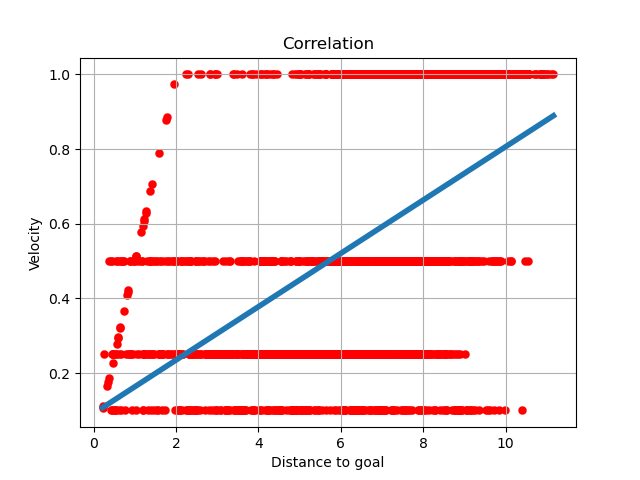
\includegraphics[width=\columnwidth]{Figure_1.png}
    \caption{Relationship between distance to the goal and expert linear
    velocity. The point cloud shows the stored expert commands, while the
    straight line represents the fitted linear regression.}
    \label{fig:linear_regression}
\end{figure}

\subsection{Interpretation of the Regression Plot}

Figure~\ref{fig:linear_regression} is not a purely linear point cloud. Several
horizontal bands are clearly visible because the expert does not always
compute the velocity with one continuous formula. During obstacle avoidance,
the reactive rules assign discrete speeds such as $0.1$, $0.25$, or $0.5$.
In free space, the saturated proportional controller produces many samples at
$v=1.0$.

Consequently, two samples may have similar goal distances but very different
expert velocities. For example,

\[
\begin{aligned}
    d\approx 6,\ \text{no obstacle}
    &\Rightarrow v\approx 1.0,\\
    d\approx 6,\ \text{frontal obstacle}
    &\Rightarrow v\approx 0.1.
\end{aligned}
\]

The regression model receives only $d$. It does not receive the sensor
measurements and therefore cannot distinguish between these two situations.
The fitted line represents an average tendency rather than a perfect
imitation of the expert controller.

\section{Why Linear Regression Fails with Saturation and Rules}

A one-dimensional linear model has the form

\[
    \hat{v}=wd+b.
\]

This function changes uniformly with distance. The expert policy, however,
contains important nonlinearities.

The first is speed saturation:

\begin{equation}
    v=\min(K_v d,v_{\max}).
    \label{eq:nonlinear_saturation}
\end{equation}

The command initially grows with distance and then becomes constant at
$v_{\max}$. One straight line cannot reproduce both the increasing region and
the saturated region exactly.

The second nonlinearity comes from the reactive obstacle-avoidance rules. The
expert velocity depends not only on distance, but also on the sensor state:

\begin{equation}
    v=f(d,s_L,s_R,s_F).
    \label{eq:expert_feature_dependence}
\end{equation}

The regression experiment instead uses

\begin{equation}
    \hat{v}=f(d).
    \label{eq:reduced_feature_dependence}
\end{equation}

Important explanatory variables are therefore missing. The largest errors
occur in situations where goal distance alone is insufficient to explain the
expert action. The limitation comes from both the restricted input and the
linear form of the model.

\section{Conclusion}

The dataset-generation stage provides the bridge between classical reactive
robotics and supervised learning. Starting from an expert controller based on
geometry, range sensing, and programmed rules, $2000$ valid independent
samples are generated. Each sample describes a robot situation and the action
that the expert would take.

Linear regression then uses this dataset to fit a first learned model for the
relationship

\[
    \texttt{distance\_to\_goal}
    \longrightarrow
    v.
\]

The fitted line learns a general trend, but it cannot reproduce the complete
expert policy. The speed saturation creates a piecewise relationship, and the
reactive obstacle rules introduce different velocities for similar goal
distances. Because the model does not receive the sensor readings, these
situations are indistinguishable from its point of view.

This limitation is the central result of the experiment rather than a failure
of the learning process. The natural next step is to provide additional
features such as $e_\theta$, $s_L$, $s_R$, and $s_F$, or to use nonlinear
models capable of approximating the expert policy more accurately.

\section{Project Task}

Generate a supervised navigation dataset by sampling independent valid robot
states in a two-dimensional environment. For each state, compute the goal
distance, normalized angular error, and left, right, and front sensor
readings. Use the existing reactive navigation controller as an expert to
assign the labels $v$ and $\omega$, and store the resulting state-perception
to-action mappings in a CSV file. Then use only \texttt{distance\_to\_goal}
as the input of a one-dimensional linear regression model for predicting the
expert velocity $v$. Compute the slope and intercept in closed form, evaluate
the predictions with MSE and MAE, plot the expert samples together with the
regression line, and explain why saturation and obstacle-dependent rules
cannot be represented accurately by a single linear feature.

% =================================================
\end{document}
% =================================================